\documentclass{article}

\usepackage{color,amsmath,amssymb,graphicx,fancyhdr,amsfonts,amsthm,verbatim,bbold,environ}
\usepackage{hyperref}
\usepackage{mkolar_definitions}
\usepackage{multirow}
\usepackage{diagbox}
\usepackage{longtable,booktabs}
\usepackage[left=2cm,top=2cm,right=2cm]{geometry}
\usepackage{listings}
% \numberwithin{algorithm}{section}


\newcommand{\tightlist}{%
  \setlength{\itemsep}{0pt}\setlength{\parskip}{0pt}}


%%%%%%%%%%%%%%%%%%%%%%%%%%%%%
\newcommand{\tta}{\theta}
\newcommand{\lag}{\left\langle}
\newcommand{\rag}{\right\rangle}
\newcommand{\lnorm}{\left\|}
\newcommand{\rnorm}{\right\|}
%%%%%%%%%%%%%%%%%%%%%%%%%%%%%
\usepackage[no-math]{fontspec}

\newfontfamily\monaco{Menlo}
\lstset{basicstyle=\footnotesize\monaco,breaklines=true}


\usepackage[ruled,lined,boxed,linesnumbered]{algorithm2e}


\title{EE357 Computer Networks Lab 3}
\author{Zhou Litao 518030910407 F1803016}
\date{\today , Spring Semester}
\begin{document}
\maketitle

%%%%%%%%%%%%%%%%%%%%%%%%%%%%%%%%%%%%%%%%%%
%%%%%%%%%%%%%                 %%%%%%%%%%%%
%%%%%%%%%%%%%    EXERCISE 1   %%%%%%%%%%%%
%%%%%%%%%%%%%                 %%%%%%%%%%%%
%%%%%%%%%%%%%%%%%%%%%%%%%%%%%%%%%%%%%%%%%%
\begin{exercise}[]{Chatting room with multiple users: client-server model with TCP protocol (50 points)

  The workflow of this chatting room is as follows: Each client can always input a message into its terminal to send it to the server. The server is responsible for receiving the message from one client and then distributing the message to other clients, such that all the messages from clients can be displayed on each client’s terminal. (In Mininet, the command to open the terminal of host h1 is ‘xterm h1’.)
    }

\noindent\emph{Solution.}

  We set up the network using \texttt{sudo python3 net.py}. It will create a network and enter the mininet terminal mode. We can run the server/client program by \texttt{xterm h1}, ... , \texttt{xterm h4}.
  
  The implementation of server is basically an extension of Beej's \emph{cheezy multiperson chat server}, which makes use of the \texttt{select()} socket API to support multi-user connection. \texttt{select()} gives us the power to monitor several sockets at the same time. It’ll tell us which ones are ready for reading, and which are ready for writing. By maintaining a set of socket file descriptors and use \texttt{select()} to choose from them, we can write codes for listening, sending and building connections in separate branches.

  We augment Beej's codes so that when a client joins or exits the room, a message will be sent to all users. Below codes use the connection close as an example. Once receive buffer returns \texttt{NULL}, the server will notify every user with the message stored in \texttt{id\_msg} buffer.

\begin{lstlisting}[language=C]
char id_msg[INET6_ADDRSTRLEN + 256 +5];
// temp buffer for packing messages for send()
...
else {
  // handle data from a client
  if ((nbytes = recv(i, buf, sizeof buf, 0)) <= 0) {
    // got error or connection closed by client
    if (nbytes == 0) {
      // connection closed
      printf("selectserver: socket %d hung up\n", i);
      // we should notify other users
      for (j = 0; j <= fdmax; j++) {
        // send to everyone!
        if (FD_ISSET(j, &master)) {
          // except the listener and ourselves
          if (j != listener && j != i) {
            memset(id_msg, 0, sizeof id_msg);
            strcat(id_msg, "INFO: ");
            strcat(
                id_msg,
                inet_ntop(remoteaddr.ss_family,
                          get_in_addr((struct sockaddr *)&remoteaddr),
                          remoteIP, INET6_ADDRSTRLEN));
            strcat(id_msg, " left the room\n");
            if (send(j, id_msg, strlen(id_msg), 0) == -1) {
              perror("send");
            }
          }
        }
      }
    } else {
      perror("recv");
    }
    close(i);            // bye!
    FD_CLR(i, &master);  // remove from master set
    free(remoteIPs[i]);
  } ...
\end{lstlisting}
  
In addition, our server now supports returning the message with the sender's IP. To achieve this, we need to maintain a mapping from socket file descriptors to the actual IP addresses. IP addresses are obatined when a connection is built. Everytime a new message comes, the server will look up the name of the sender from the mapping.

\begin{lstlisting}[language=C]
#define MAX_FD_NUM 64
...
char *remoteIPs[MAX_FD_NUM];  // remoteIPs
...
if (i == listener) {
  // handle new connections
  addrlen = sizeof remoteaddr;
  newfd = accept(listener, (struct sockaddr *)&remoteaddr, &addrlen);
  inet_ntop(remoteaddr.ss_family,
            get_in_addr((struct sockaddr *)&remoteaddr), remoteIP,
            INET6_ADDRSTRLEN);
  remoteIPs[newfd] =
      (char *)malloc((strlen(remoteIP) + 1) * sizeof(char));
  strcpy(remoteIPs[newfd], remoteIP);
  ...

...
else {
  // we got some data from a client
  for (j = 0; j <= fdmax; j++) {
    // send to everyone!
    if (FD_ISSET(j, &master)) {
      // except the listener and ourselves
      if (j != listener && j != i) {
        memset(id_msg, 0, sizeof id_msg);
        strcat(id_msg, remoteIPs[i]); // remoteIP is looked up and sent
        strcat(id_msg, ": ");
        strncat(id_msg, buf, strlen(buf));
        if (send(j, id_msg, strlen(id_msg), 0) == -1) {
          perror("send");
        }
      }
    }
  }
  memset(buf, 0, sizeof buf); /* IMPORTANT! */
}
}  // END handle data from client
\end{lstlisting}

  As for the client, it should be able to read and write to a socket file descriptor simultaneously. We use \texttt{fork()} to address this problem. To be specific, after we obatin the file descriptor, the process will be forked into two processes, one for reading from \texttt{stdin} and writing to the socket, while the other for monitoring the socket and print to \texttt{stdout} once a message comes. We leave out the codes for building sockets and present the codes after \texttt{fork()} as follows.

\begin{lstlisting}[language=C]
int main(int argc, char *argv[]) {
  int sockfd, numbytes;
  struct addrinfo hints, *servinfo, *p;
  int rv;

  ...
  freeaddrinfo(servinfo);  // all done with this structure

  pid_t pid;
  pid = fork();
  if (pid == -1) {
    error_print((char *)"fork");
  }

  if (pid == 0) {  // child process, for listening
    char recv_buf[MAXDATASIZE] = {0};

    while (1) {
      bzero(recv_buf, sizeof(recv_buf));
      int ret = read(sockfd, recv_buf, sizeof(recv_buf));
      if (ret == -1)
        error_print((char *)"read");
      else if (ret == 0) { /* server is closed */
        printf("server is close!\n");
        break;
      }
      fputs(recv_buf, stdout); /* for received message, print into stdout */
    }

    close(sockfd); /* before ending, close the socket file descriptor */
    kill(getppid(), SIGUSR1); /* should signal the father process to exit */
    exit(EXIT_SUCCESS);       /* should notify father process exit success */
  } else { // parent process, for sending
    signal(SIGUSR1, quit_tranmission); /* deal with transmission corruption */
    char send_buf[MAXDATASIZE] = {0};

    while (fgets(send_buf, sizeof(send_buf), stdin) != NULL)
    /* if the stdin is not closed */
    {
      int set = write(sockfd, send_buf, strlen(send_buf));
      /* send data to the server */
      if (set < 0) error_print((char *)"write");
      bzero(send_buf, strlen(send_buf));
    }

    close(sockfd); /* end of program, close socket file descriptor */
  }
  return 0;
}
\end{lstlisting}

Note that exceptions may occur on subprocesses (due to either user interruption or connection failure). In this case, we write some signal handlers to ensure that no dangling process exists if error occurs.

A running example of our final program is demonstrated in Figure \ref{fig:ex1}. We run \texttt{./server} in host 1 and \texttt{./client} in other hosts.


\begin{figure}[hb]
  \begin{center}
  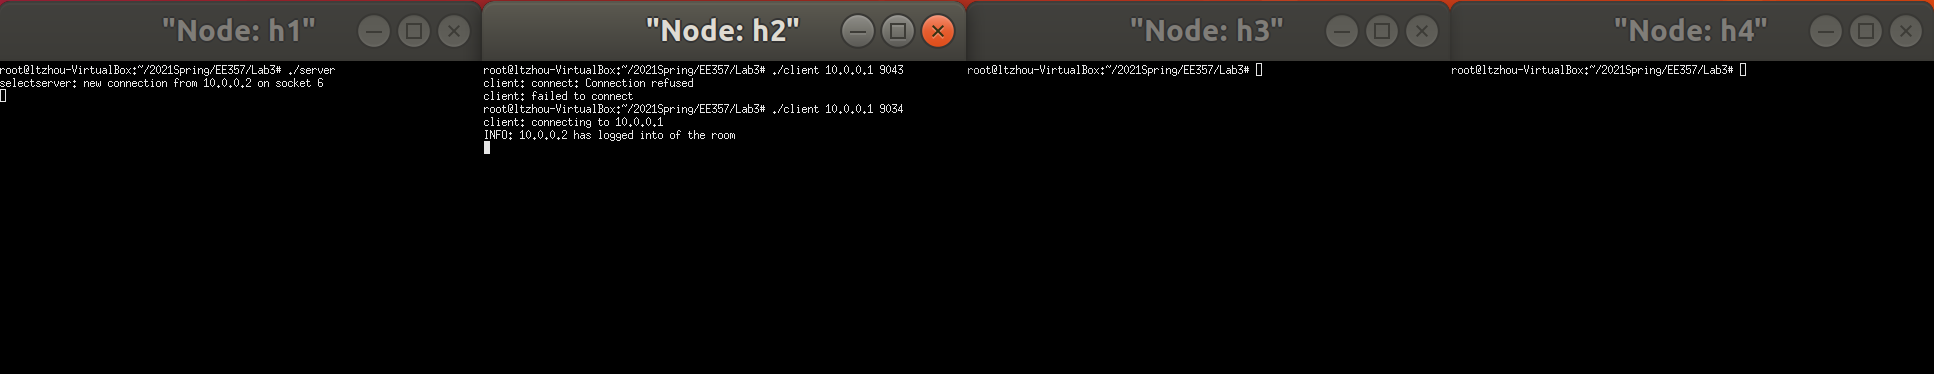
\includegraphics[width=14cm]{img/lab3/chat1.png}
  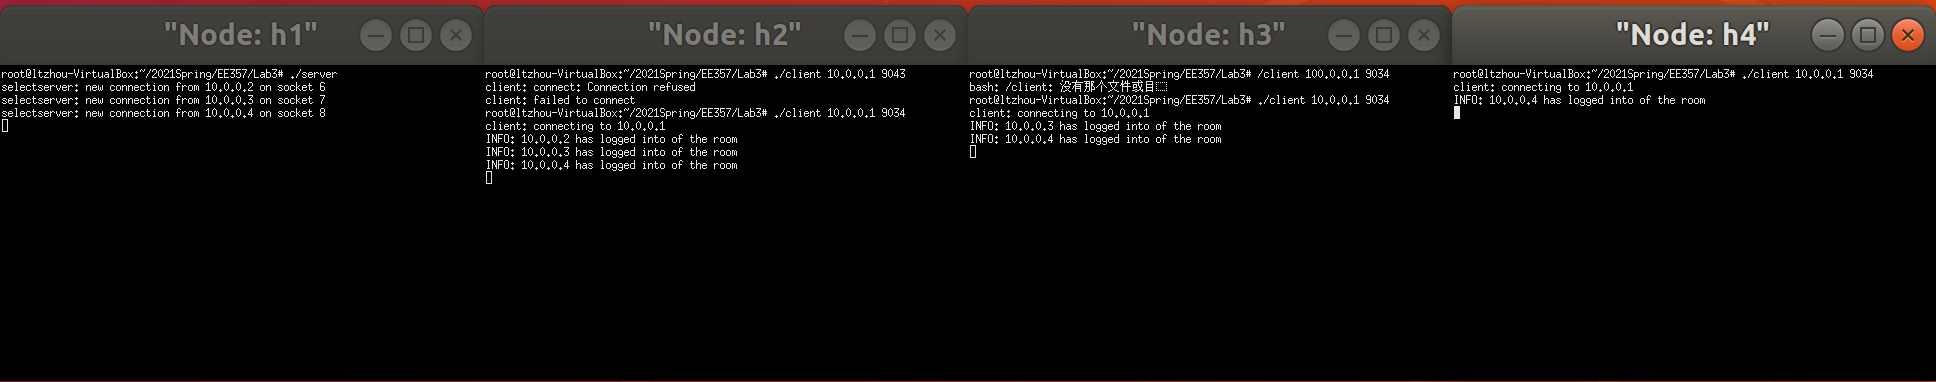
\includegraphics[width=14cm]{img/lab3/chat2.png}
  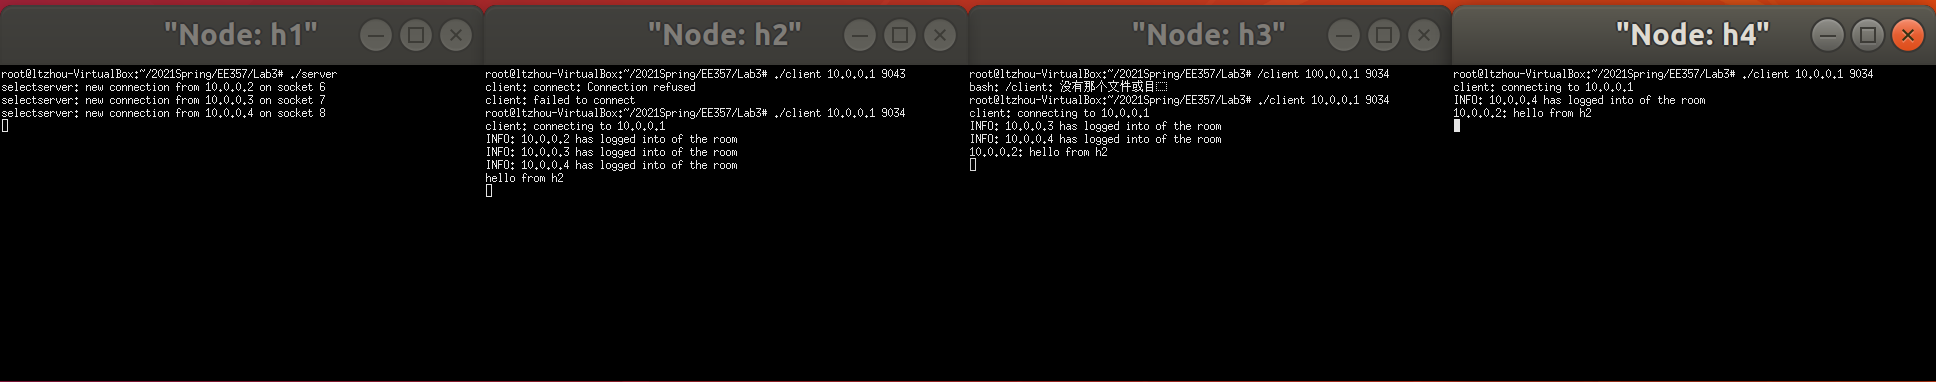
\includegraphics[width=14cm]{img/lab3/chat3.png}
  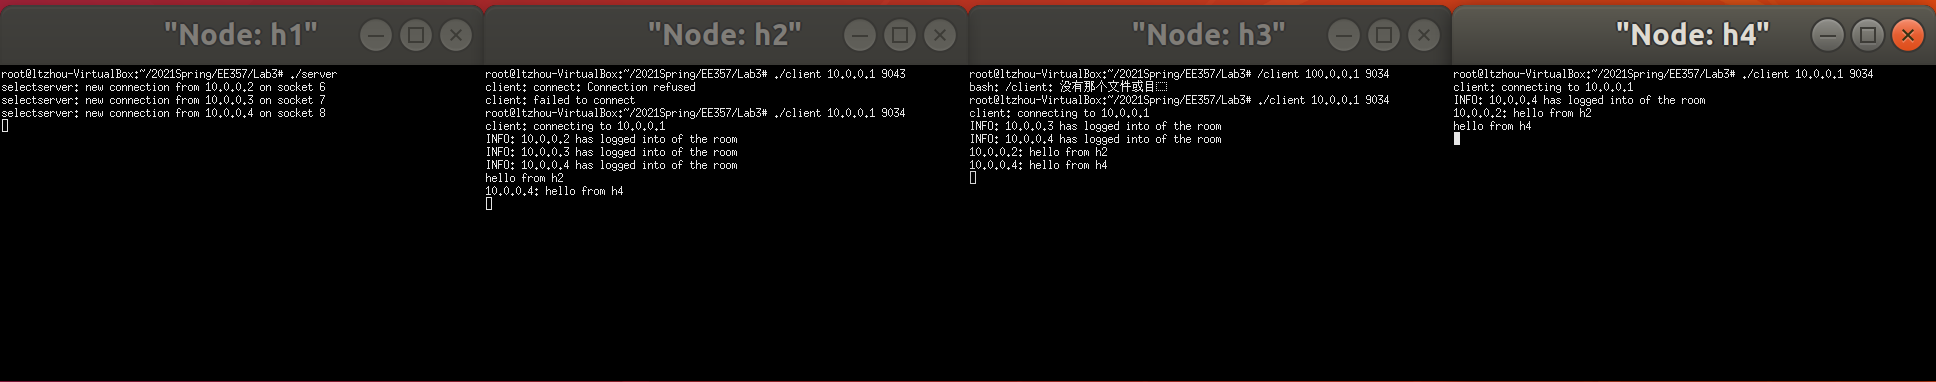
\includegraphics[width=14cm]{img/lab3/chat4.png}
  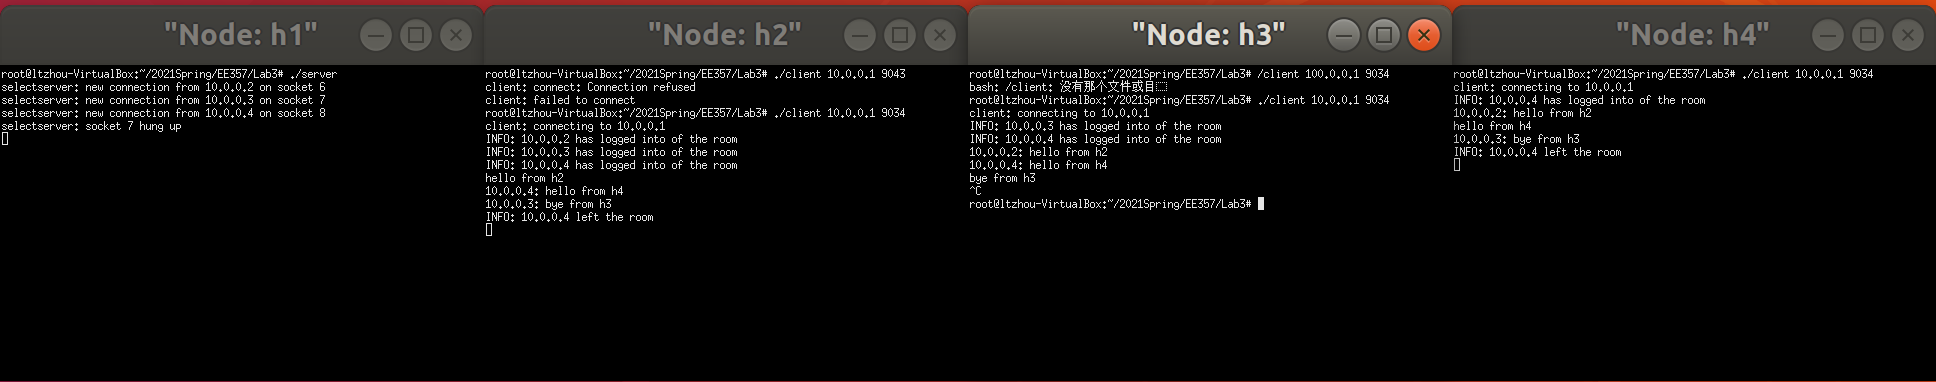
\includegraphics[width=14cm]{img/lab3/chat5.png}
  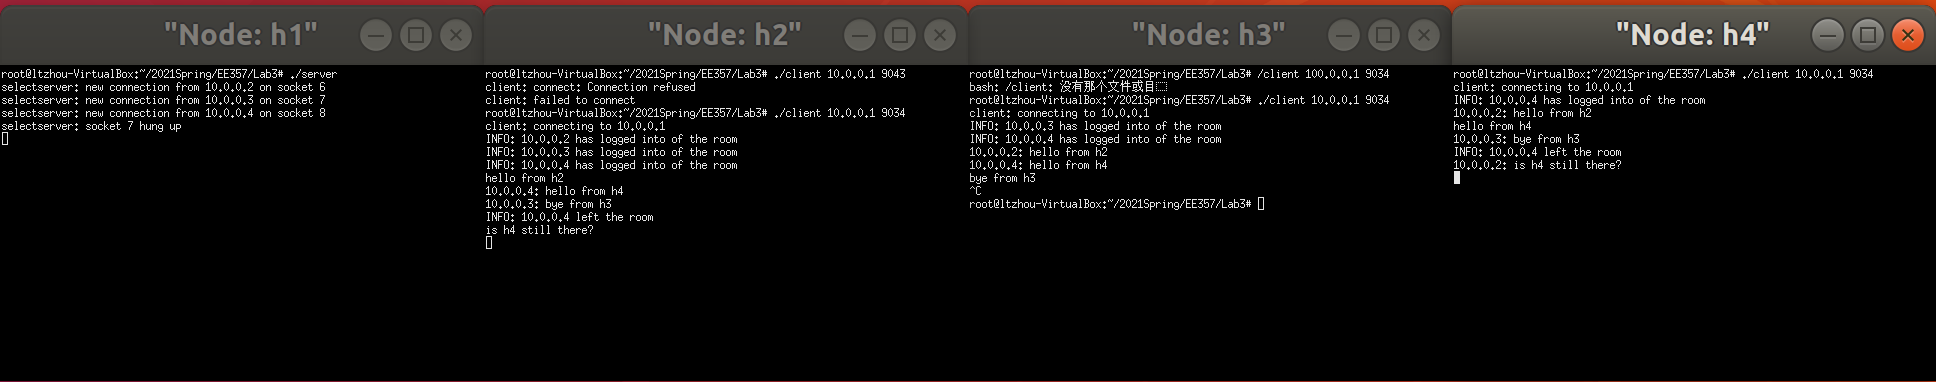
\includegraphics[width=14cm]{img/lab3/chat6.png}
  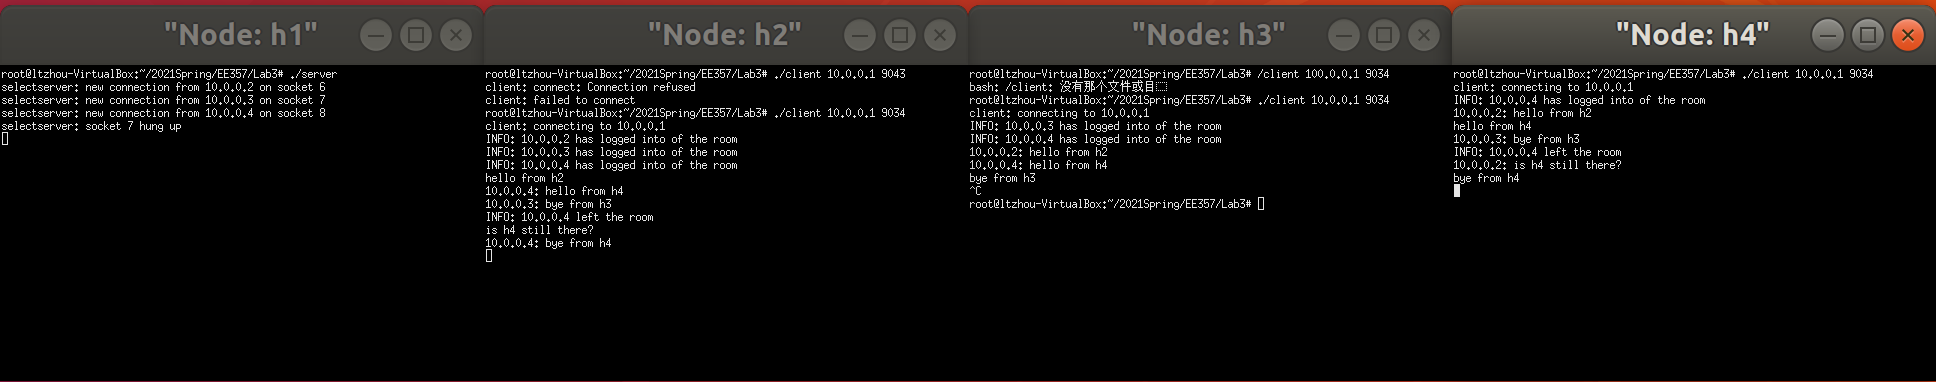
\includegraphics[width=14cm]{img/lab3/chat7.png}
  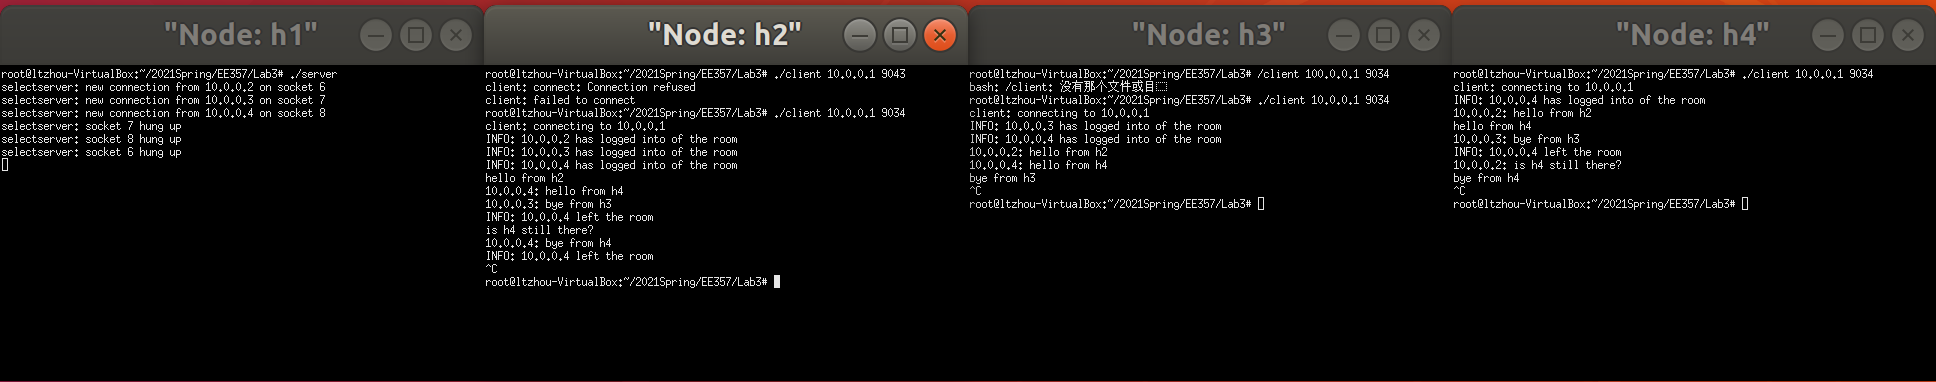
\includegraphics[width=14cm]{img/lab3/chat8.png}
  \caption{Client Server Chatting Room Demo}
  \label{fig:ex1}
  \end{center}
\end{figure}

  \label{ex1}
\end{exercise}


%%%%%%%%%%%%%%%%%%%%%%%%%%%%%%%%%%%%%%%%%%
%%%%%%%%%%%%%                 %%%%%%%%%%%%
%%%%%%%%%%%%%    EXERCISE 2   %%%%%%%%%%%%
%%%%%%%%%%%%%                 %%%%%%%%%%%%
%%%%%%%%%%%%%%%%%%%%%%%%%%%%%%%%%%%%%%%%%%
\begin{exercise}[]{Chatting room with multiple users: client-only model with UDP protocol (50 points)
  
  The workflow of this chatting room is as follows: Each client can send the message to the broadcast address. At the same time, they also continuously listen to the messages from the broadcast address. In such way, each client can transmit/receive messages to/from other clients without the help of a server. All the messages from clients should be displayed on each client’s terminal.

  }

\noindent\emph{Solution.}

We refer to Beej's implementation of \texttt{talker.c} and \texttt{listener.c}, where \texttt{listener} sits on a machine waiting for an incoming packet on port 4950. \texttt{talker} sends a packet to that port, on the specified machine, that contains whatever the user enters on the command line. To merge them into one single program, we write our code in a \texttt{fork()} style.

Note, however, here the listener process and the talker process do not share a same socket descriptor. The listener should listen to the designated port on its local machine, while the talker should send to the designated ports of every machine in the network. We choose to move the socket creation phase into the forked subprocesses.

The implementation of the listener subprocess is as follows. The body of the subprocess basically follows the rountine in Beej's \texttt{listener.c}


\begin{lstlisting}[language=C]
int main(int argc, char *argv[]) {
  struct addrinfo hints;

  int listenfd;
  int rv;
  int numbytes;
  int host_idx;
  int talkfd[HOST_NUM];

  if (argc != 1) {
    fprintf(stderr, "usage: %s\n", argv[0]);
    exit(1);
  }

  pid_t pid;
  pid = fork();
  if (pid == -1) {
    error_print((char *)"fork");
  }

  if (pid == 0) {  // listener
    struct addrinfo *servinfo, *p;
    memset(&hints, 0, sizeof hints);
    hints.ai_family = AF_INET;  // set to AF_INET to use IPv4
    hints.ai_socktype = SOCK_DGRAM;
    hints.ai_flags = AI_PASSIVE;  // use my IP
    if ((rv = getaddrinfo(NULL, SERVERPORT, &hints, &servinfo)) != 0) {
      fprintf(stderr, "getaddrinfo: %s\n", gai_strerror(rv));
      return 1;
    }

    // loop through all the results and make a socket
    ...
    // and bind listenfd to p 
    freeaddrinfo(servinfo);
    struct sockaddr_storage their_addr;
    char buf[MAXDATASIZE];
    socklen_t addr_len;
    char s[INET6_ADDRSTRLEN];
    while (1) {
      addr_len = sizeof their_addr;
      if ((numbytes = recvfrom(listenfd, buf, MAXDATASIZE - 1, 0,
                               (struct sockaddr *)&their_addr, &addr_len)) ==
          -1) {
        error_print((char *)"recvfrom");
      } else if (numbytes == 0) {
        printf("server is close!\n");
        break;
      }
      buf[numbytes] = '\0';
      printf(
          "%s : %s",
          inet_ntop(their_addr.ss_family,
                    get_in_addr((struct sockaddr *)&their_addr), s, sizeof s),
          buf);
      bzero(buf, strlen(buf));
    }
    close(listenfd); /* before ending, close the socket file descriptor */
    kill(getppid(), SIGUSR1); /* should signal the father process to exit */
    exit(EXIT_SUCCESS);       /* should notify father process exit success */
  } ... 
\end{lstlisting}

  As for the sender, we should change the original 1-to-1 sender in Beej's \texttt{talker.c} into 1-to-4 sender structure in our network. Therefore, we maintain a configure table \texttt{network\_ips} in the program. We will build four separate talker file descriptors for each IP address in the configuration table. As a result, the \texttt{talkerfd} and \texttt{p} variable in the original program should be changed into an array of \texttt{talkerfd}s and \texttt{p}s. We modify Beej's \texttt{talker.c} and implement the sender process as follows.

\begin{lstlisting}[language=C]
const char *network_ips[] = {"10.0.0.1", "10.0.0.2", "10.0.0.3", "10.0.0.4"};

#define HOST_NUM 4

... else {                    // talker process
  signal(SIGUSR1, quit_tranmission); /* deal with transmission corruption */
  memset(&hints, 0, sizeof hints);
  hints.ai_family = AF_INET;  // set to AF_INET to use IPv4
  hints.ai_socktype = SOCK_DGRAM;

  pid_t ppid;

  struct addrinfo *servinfo[HOST_NUM], *p[HOST_NUM];

  for (host_idx = 0; host_idx < HOST_NUM; ++host_idx) {
    if ((rv = getaddrinfo(network_ips[host_idx], SERVERPORT, &hints,
                          &(servinfo[host_idx]))) != 0) {
      fprintf(stderr, "getaddrinfo: %s\n", gai_strerror(rv));
      return 1;
    }

    // loop through all the results and make a socket
    ...
    // p[host_idx] is updated
  }

  char send_buf[MAXDATASIZE] = {0};

  while (fgets(send_buf, sizeof(send_buf), stdin) != NULL)
  /* if the stdin is not closed */
  {
    for (int i = 0; i < HOST_NUM; ++i) {
      if ((numbytes = sendto(talkfd[i], send_buf, strlen(send_buf), 0,
                            (p[i])->ai_addr, (p[i])->ai_addrlen)) == -1) {
        error_print((char *)"sendto");
      }
    }
    bzero(send_buf, strlen(send_buf));
  }
  for (int i = 0; i < HOST_NUM; ++i) {
    freeaddrinfo(servinfo[i]);
    close(talkfd[i]); /* end of program, close socket file descriptor */
  }
}
\end{lstlisting}


A running example of our final program is demonstrated in Figure \ref{fig:ex2}. We run \texttt{./udpclient} on four hosts.


\begin{figure}[hb]
  \begin{center}
  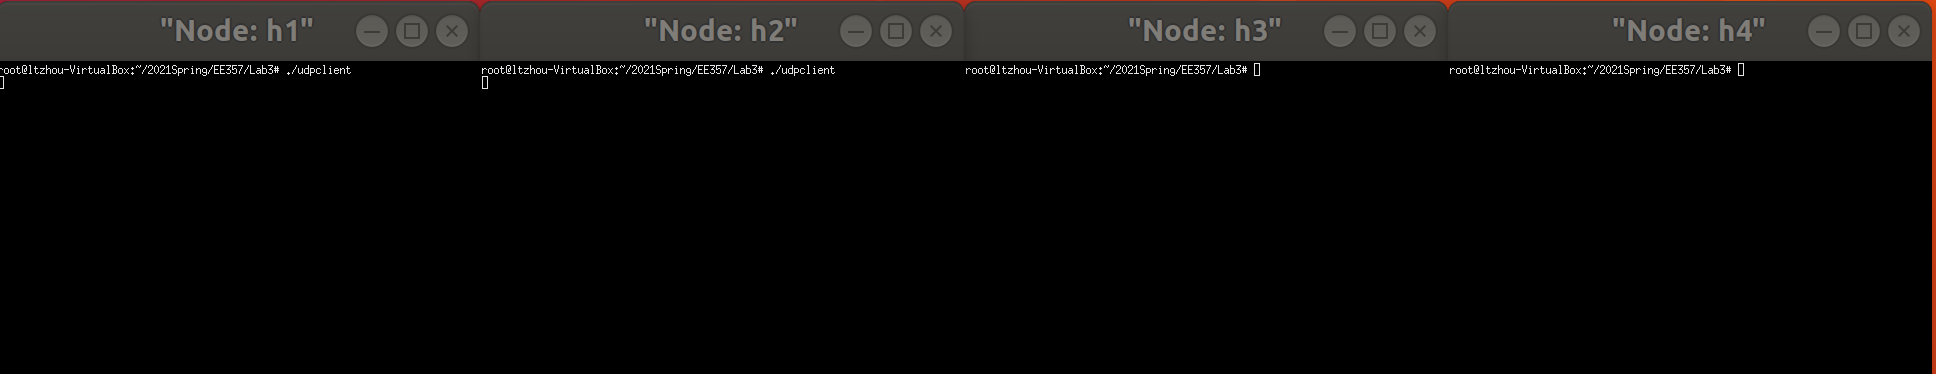
\includegraphics[width=14cm]{img/lab3/udpchat1.png}
  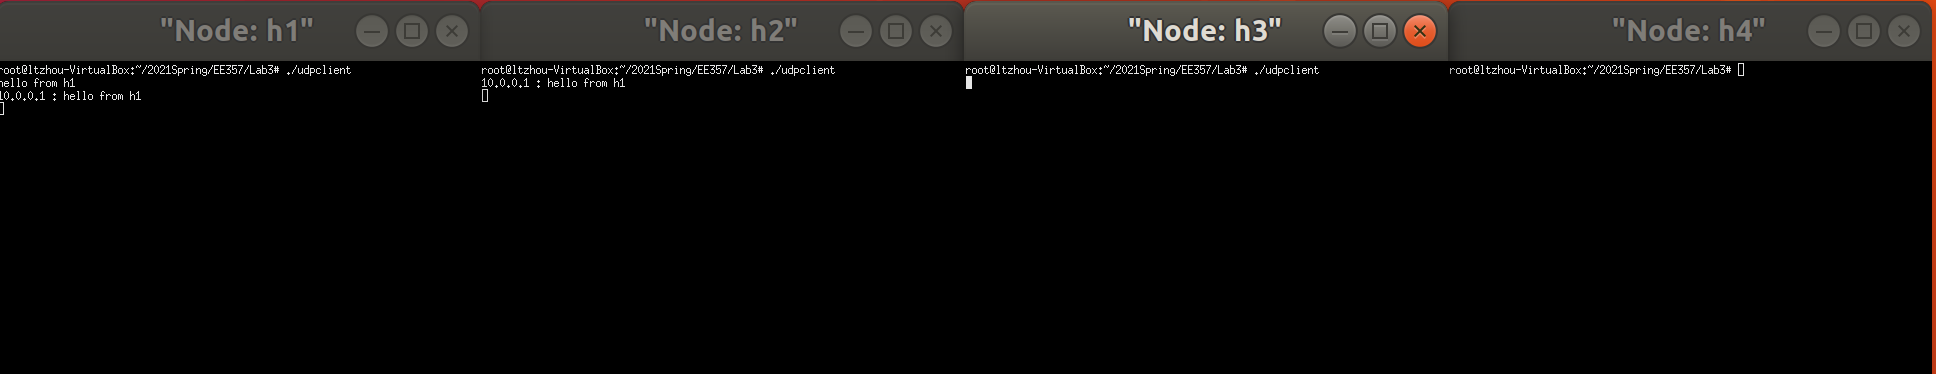
\includegraphics[width=14cm]{img/lab3/udpchat2.png}
  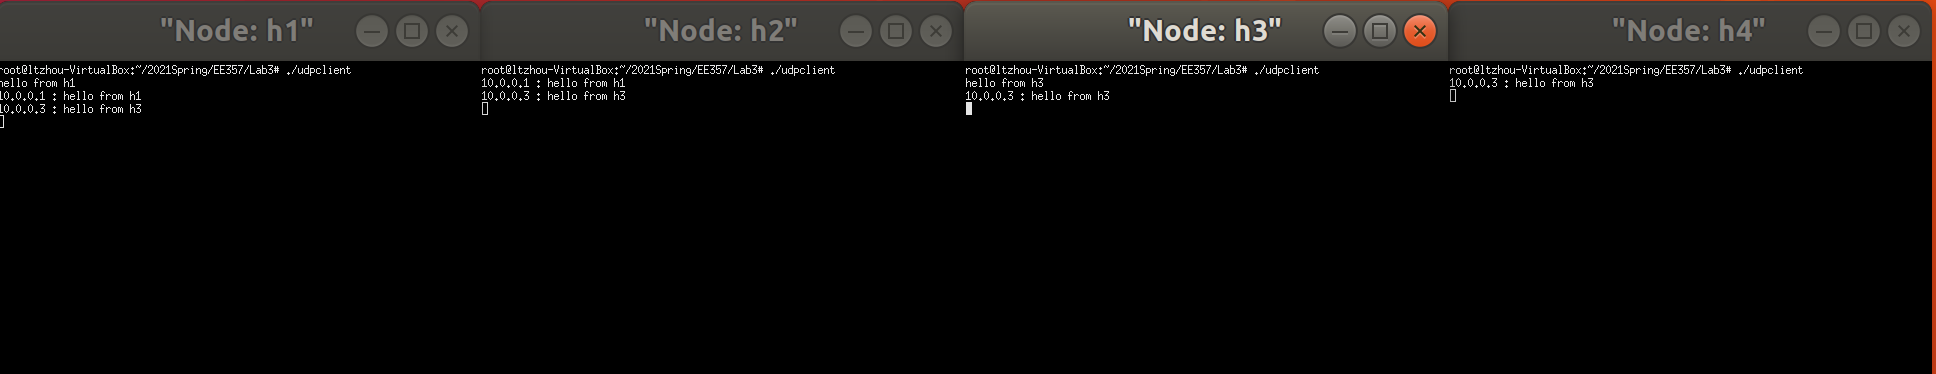
\includegraphics[width=14cm]{img/lab3/udpchat3.png}
  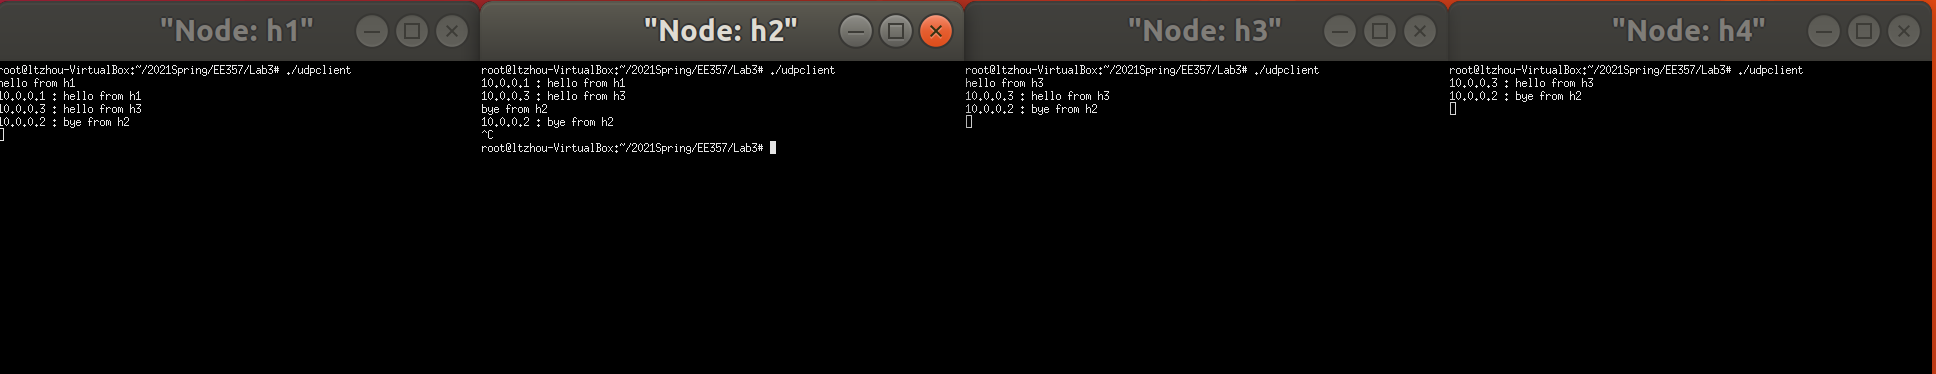
\includegraphics[width=14cm]{img/lab3/udpchat4.png}
  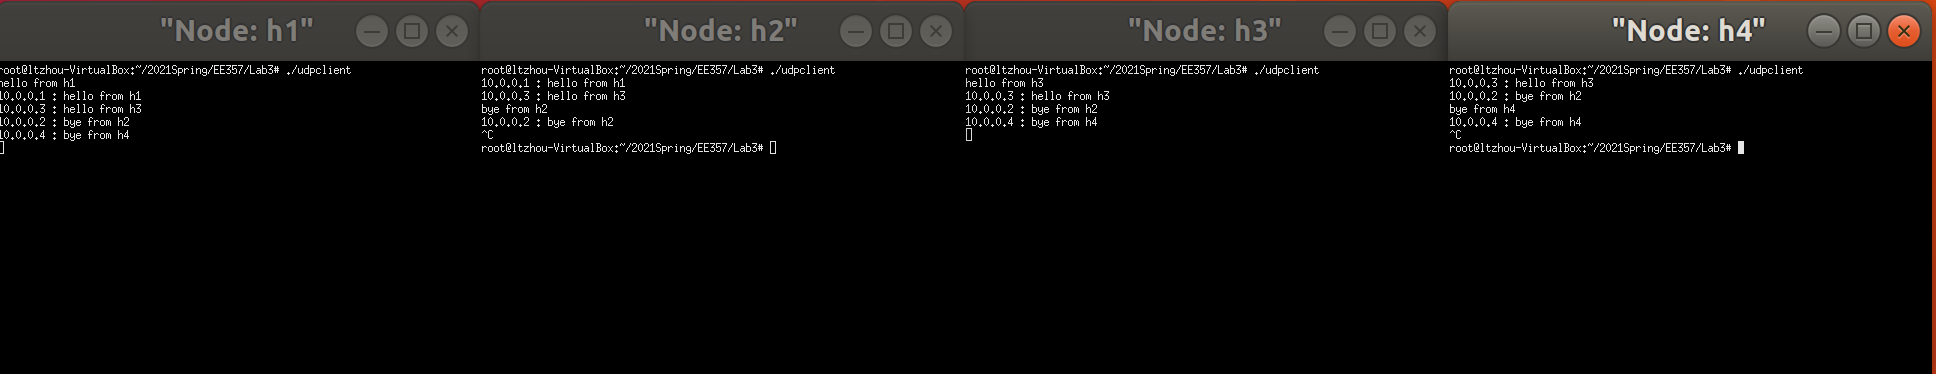
\includegraphics[width=14cm]{img/lab3/udpchat5.png}
  \caption{UDP Chatting Room Demo}
  \label{fig:ex2}
  \end{center}
\end{figure}

\label{ex2}
\end{exercise}

%%%%%%%%%%%%%%%%%%%%%%%%%%%%%%%%%%%%%%%%%%
%%%%%%%%%%%%%                 %%%%%%%%%%%%
%%%%%%%%%%%%%    EXERCISE 3   %%%%%%%%%%%%
%%%%%%%%%%%%%                 %%%%%%%%%%%%
%%%%%%%%%%%%%%%%%%%%%%%%%%%%%%%%%%%%%%%%%%
\begin{exercise}[]{Bonus question:For each client that you built in the above Question 2, it will receive the messages sent by itself from the broadcast address. Can you filter out these messages, such that each client’s terminal will not display the message sent by the client itself? Bonus will be offered, if you could realize this function. }
  
My solution is to avoid sending messages to the host itself. Since the public IP address cannot be directly obtained from the socket file descriptor, we choose to let the user pass an argument indicating the host number it has (i.e. the host it want to filter out) when running \texttt{./udpchat}. Its implementation is demonstrated as follows.


\begin{lstlisting}[language=C]
int main(int argc, char *argv[]) {
  struct addrinfo hints;

  int listenfd;
  int rv;
  int numbytes;
  int host_idx;
  int talkfd[HOST_NUM];
  int self; // <-- This is new

  if (argc != 2) {
    fprintf(stderr, "usage: %s <your declared host number> \n", argv[0]);
    exit(1);
  }

  sscanf(argv[1], "%d", &self); / <-- This is new

  pid_t pid;
  pid = fork();
  if (pid == -1) {
    error_print((char *)"fork");
  }

  if (pid == 0) {  // listener
    ... // create socket
    while (1) {
      addr_len = sizeof their_addr;
      if ((numbytes = recvfrom(listenfd, buf, MAXDATASIZE - 1, 0,
                               (struct sockaddr *)&their_addr, &addr_len)) ==
          -1) {
        error_print((char *)"recvfrom");
      } else if (numbytes == 0) {
        printf("server is close!\n");
        break;
      } // receive message
      if (strcmp(inet_ntop(their_addr.ss_family,
                           get_in_addr((struct sockaddr *)&their_addr), s,
                           sizeof s),
                 network_ips[self]) != 0) {
      // <-- This is new, filter out message from self address
        buf[numbytes] = '\0';
        printf(
            "%s : %s",
            inet_ntop(their_addr.ss_family,
                      get_in_addr((struct sockaddr *)&their_addr), s, sizeof s),
            buf);
      }
      bzero(buf, strlen(buf));
    }
    close(listenfd); /* before ending, close the socket file descriptor */
    kill(getppid(), SIGUSR1); /* should signal the father process to exit */
    exit(EXIT_SUCCESS);       /* should notify father process exit success */
  } ...
  return 0;
}
\end{lstlisting}



A running example of our final program is demonstrated in Figure \ref{fig:ex3}. We run \texttt{./udpchat} on four hosts.


\begin{figure}[hb]
  \begin{center}
  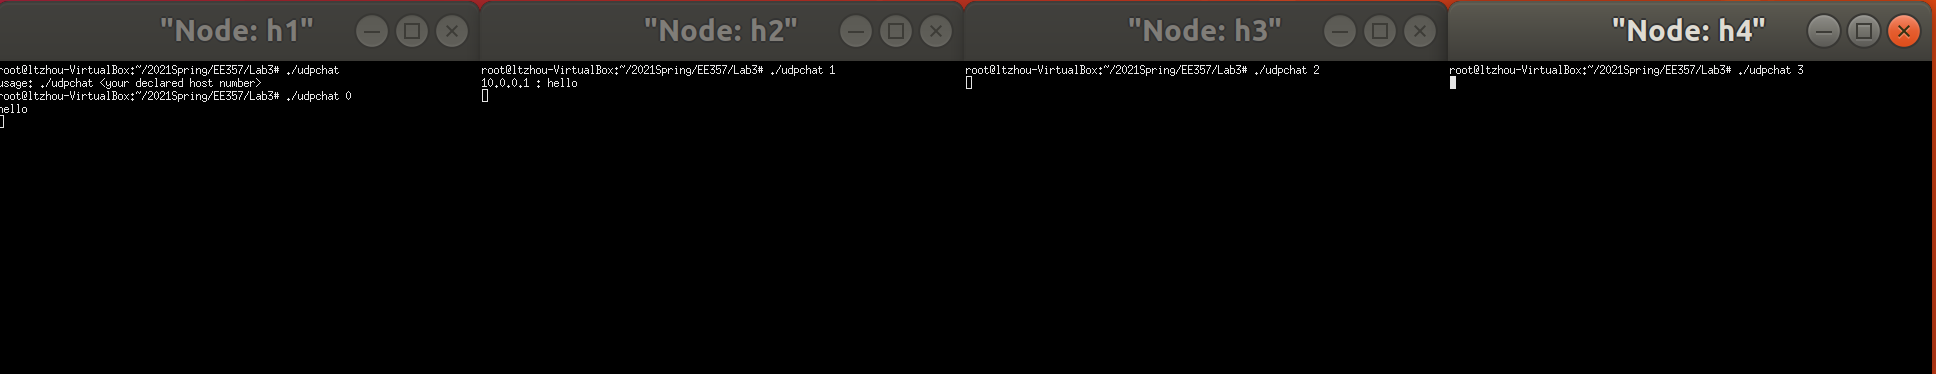
\includegraphics[width=14cm]{img/lab3/udpadv1.png}
  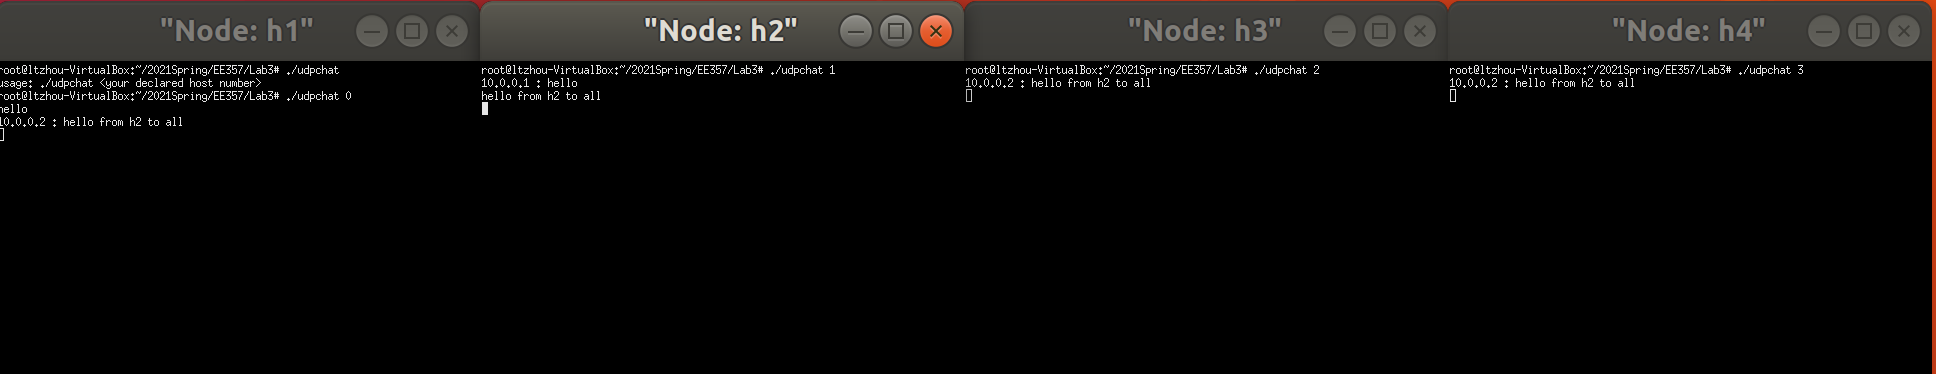
\includegraphics[width=14cm]{img/lab3/udpadv2.png}
  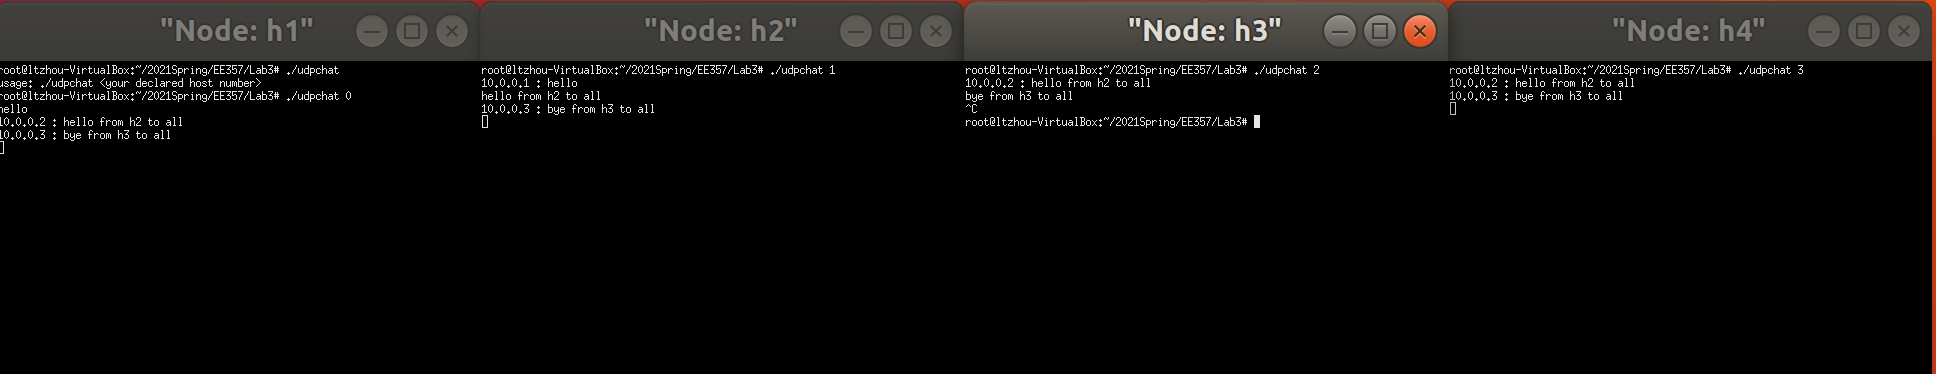
\includegraphics[width=14cm]{img/lab3/udpadv3.png}
  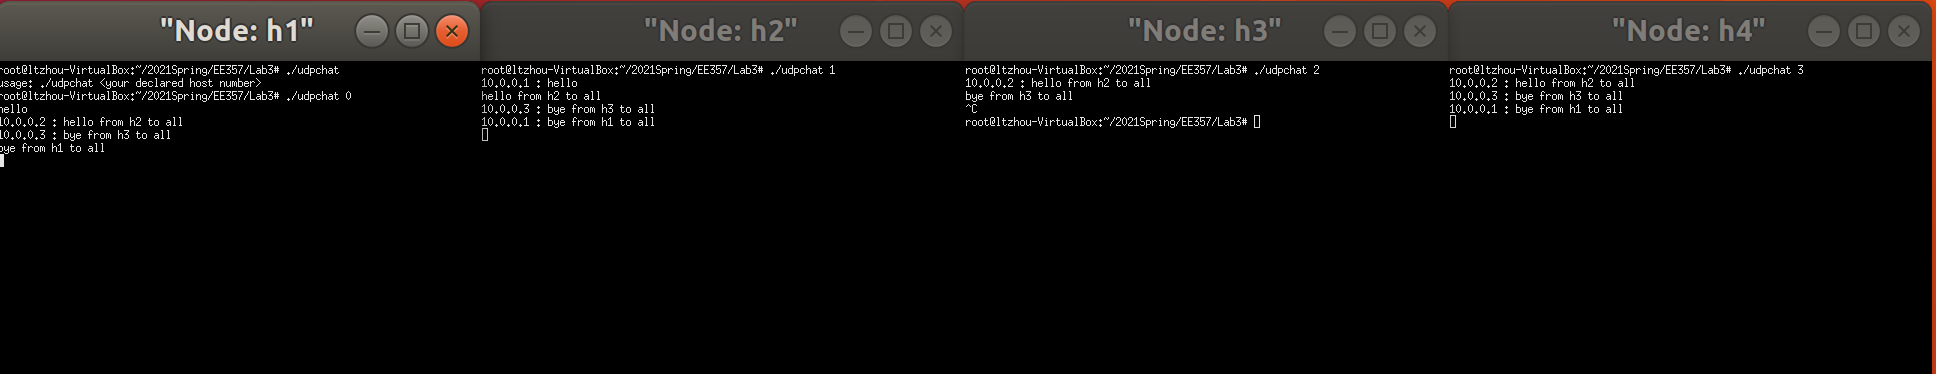
\includegraphics[width=14cm]{img/lab3/udpadv4.png}
  \caption{Advanced UDP Chatting Room Demo}
  \label{fig:ex3}
  \end{center}
\end{figure}

  \label{ex3}
\end{exercise}



\appendix

\section{References}

\begin{enumerate}
  \item Zapałowski, Bartosz. "Beej’s Guide to Network Programming." (1995).
  \item Linux based Socket programming - TCP full duplex Server-Client chat program 
  
  {\ttfamily https://blog.csdn.net/Apollon\_krj/article/details/53437764}
  \item Bryant, Randal E., and O'Hallaron David Richard. Computer systems: a programmer's perspective. Chapter 8, 11. Upper Saddle River: Prentice Hall, 2003.
\end{enumerate}


\end{document}